\documentclass[a4paper,12pt]{article} 

%%% Работа с русским языком
\usepackage{cmap}					% поиск в PDF
\usepackage{mathtext} 				% русские буквы в фомулах
\usepackage[T2A]{fontenc}			% кодировка
\usepackage[utf8]{inputenc}			% кодировка исходного текста
\usepackage[english,russian]{babel}	% локализация и переносы

%%% Дополнительная работа с математикой
\usepackage{amsmath,amsfonts,amssymb,amsthm,mathtools, gensymb} % AMS
\usepackage{icomma} % "Умная" запятая: $0,2$    ф--- число, $0, 2$ --- перечисление

%%Таблица
\usepackage[table,xcdraw]{xcolor}
\usepackage{caption}
\usepackage{floatrow}
\floatsetup[table]{capposition=top}
\floatsetup[wrapfigure]{capposition=bottom}
\usepackage{multirow}

\usepackage{hyperref}

%Отступы и поля 
\textwidth=18cm
\oddsidemargin=-1cm
\topmargin=-2cm
\textheight=25cm


%% Номера формул
\mathtoolsset{showonlyrefs=false} % Показывать номера только у тех формул, на которые есть \ref{} в тексте.

%% Шрифты
\usepackage{euscript}	 % Шрифт Евклид
\usepackage{mathrsfs} % Красивый матшрифт

%% Свои команды
\DeclareMathOperator{\sgn}{\mathop{sgn}}

%% Перенос знаков в формулах (по Львовскому)
\newcommand*{\hm}[1]{#1\nobreak\discretionary{}
{\hbox{$\mathsurround=0pt #1$}}{}}

%% Стиль страницы
\usepackage{fancyhdr}

%% Для рисунков
\usepackage{graphicx}
\usepackage[export]{adjustbox}
\usepackage{float}
\usepackage{ragged2e}
\usepackage{wrapfig}

\pagestyle{fancy}
\begin{document}
\begin{titlepage}
\begin{center}
%\vspace*{1cm}
\large{\small ФЕДЕРАЛЬНОЕ ГОСУДАРСТВЕННОЕ АВТОНОМНОЕ ОБРАЗОВАТЕЛЬНОЕ\\ УЧРЕЖДЕНИЕ ВЫСШЕГО ОБРАЗОВАНИЯ \\ МОСКОВСКИЙ ФИЗИКО-ТЕХНИЧЕСКИЙ ИНСТИТУТ\\ (НАЦИОНАЛЬНЫЙ ИССЛЕДОВАТЕЛЬСКИЙ УНИВЕРСИТЕТ)\\ ФАКУЛЬТЕТ АЭРОКОСМИЧЕСКИХ ТЕХНОЛОГИЙ}
\vfill
\line(1,0){490}\\[1mm]
\huge{Лабораторная работа 2.3/2.2}\\
\huge\textbf{Изучение спектра атома водорода и молекулы йода}\\
\line(1,0){490}\\[1mm]
\vfill
\begin{flushright}
\normalsize{Рогозин Владимир}\\
\normalsize{\textbf{Группа Б03-106}}\\
\end{flushright}
\end{center}
\end{titlepage}
\fancyhead[L] {Работа 2.3/2.2}

\textbf{Цель работы}:
Исследовать спектр поглощения паров йода в видимой области; по результатам измерения вычислить энергию колебательного кванта молекулы йода и энергию её диссоциации в основном и возбужденном состояниях.


% \textbf{Оборудование}:
% лазер; кассета с набором сеток разного
% периода; линзы; щель с микрометрическим винтом; оптический стол
% c набором рейтеров и крепёжных винтов; экран; линейка.


\section{Теоретические сведения}
Молекулы обладают более богатым спектром возбужденных состояний, чем изолированные атомы. В то время как возбуждения атомов -- это переходы их электронов на более высоко расположенные энергетические уровни, в молекулах могут возбуждаться дополнительные степени свободы: колебания составляющих их атомов друг относительно друга и вращения молекул относительно различных осей. В первом приближении энергия молекулы может быть представлена в виде
\begin{equation}\label{eq: Energy in molecule}
    E = E_\text{эл} + E_\text{колеб} + E_\text{вращ}. 
\end{equation}
Указанные возбуждения считаются независимыми. Это с хорошей точностью справедливо для малых амплитуд колебаний ядер. Аналогичное предположение делается и относительно электронных состояний: мы предполагаем, что энергия электронов мало меняется за счет колебательного движения молекулы. На языке волновых функций эти предположения означают, что волновая функция молекулы может быть представлена в виде произведения трех волновых функций, отвечающих электронным движениям, колебаниям и вращениям молекулы:
\begin{equation}\label{eq: Psi-func in molecule}
    \psi = \psi_\text{эл}\cdot\psi_\text{колеб}\cdot\psi_\text{вращ}. 
\end{equation}

\subsection{Электронные термы}
Массы ядер атомов велики по сравнению с массой электрона. Благодаря такой разнице в массах, скорости движения ядер в молекуле малы по сравнению со скоростями электронов. Это дает возможность рассматривать электронное движение при неподвижных ядрах, расположенных на определенных расстояниях друг от друга. Электронные термы молекул не отличаются по своему происхождению от электронных термов изолированных атомов, но число их значительно превышает число этих термов в атомах. Любой атом в молекуле находится в электрическом поле остальных ее атомов, о таком поле говорят «внутреннее электрическое поле». Следует, однако, отметить, что при соединении атомов в молекулу заполненные оболочки атомов мало меняются. Существенно может измениться только распределение электронной плотности в не до конца заполненных оболочках.

\subsection{Колебательные возбуждения}
При смещении атомов в молекуле из равновесных положений могут возникать их колебания около положения равновесия. Силы, обеспечивающие устойчивость молекулы, имеют электрическую природу. На ближних расстояниях атомы, образующие молекулы, отталкиваются, и обусловлено это кулоновским отталкиванием сближающихся ядер. На больших расстояниях атомы притягиваются -- это может происходить за счет кулоновского притяжения разноименных ионов (ионные молекулы) либо за счет обменных сил, имеющих квантово-механическую природу (атомные молекулы). В результате образуется потенциальный минимум, как показано на рис. \hyperref[fig: Oscillation energy levels]{1}.
\begin{figure}[H]\label{fig: Oscillation energy levels}
    \centering
    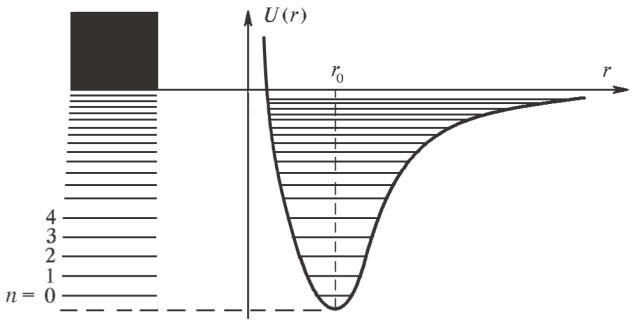
\includegraphics[width = 0.9\textwidth]{Oscillation energy levels.png}
    \caption{Схема энергетических уровней двухатомной молекулы}
\end{figure}

Вблизи минимума кривая потенциальной энергии $U(r)$ мало отличается от параболы и нижние уровни энергии близки к уровням гармонического осциллятора. Слева на рис. \hyperref[fig: Oscillation energy levels]{1} показана схема энергетических уровней молекулы, зачерненная часть соответствует непрерывному спектру, расположенному выше энергии диссоциации молекулы. Энергия колебаний атомов молекулы квантуется:
\begin{equation}\label{eq: Oscillation energy}
    E_\text{колеб} = \hbar\omega_0\left(n + \frac{1}{2}\right) - \hbar\omega_0 x_n\left(n + \frac{1}{2}\right)^2.
\end{equation}
Здесь первое слагаемое -- энергия гармонического осциллятора с собственной частотой $\omega_0$ , $n = 0, 1, 2, . . .$ -- колебательное квантовое число. Второе слагаемое учитывает отступление от гармонического закона колебаний. Обычно $x_n$ -- коэффициент ангармонизма -- мал, и второе слагаемое существенно при больших $n$, т. е. при больших амплитудах колебаний ядер. Таким образом, при небольших $n$ имеем систему энергетических уровней гармонического осциллятора:
\begin{equation}\label{eq: Oscillation energy simplified}
    E_\text{колеб} = \hbar\omega_0\left(n + \frac{1}{2}\right).
\end{equation}

Из оценки следует, что
\begin{equation}\label{eq: Oscillation energy contribution}
    \frac{\omega_\text{колеб}}{\omega_\text{эл}} \approx \sqrt{\frac{m}{M}}.
\end{equation}
Для средних ядер $A \approx 100$ получаем оценку
\begin{equation}\label{eq: Oscillation energy contribution estimate}
    \frac{\omega_\text{колеб}}{\omega_\text{эл}} \approx 2 \cdot 10^{-3}.
\end{equation}
Эта оценка показывает, насколько мал квант колебательной энергии по сравнению с расстоянием между электронными возбуждениями.

\subsection{Вращательные возбуждения}
У каждой молекулы имеется система дискретных состояний, соответствующих ее вращению как целого вокруг некоторой оси. Для оценки характерных частот вращательного движения рассмотрим двухатомную молекулу с массами атомов M и межатомным расстоянием $a_0$. Пусть ось вращения проходит посредине между атомами и перпендикулярна оси молекулы, т. е. вращения происходят относительно центра масс молекулы. Момент инерции относительно этой оси
\begin{equation}\label{eq: Momentum of inertia}
    J \approx Ma_0^2.
\end{equation}
Энергия вращения квантуется и равна
\begin{equation}\label{eq: Rotation energy}
    E_\text{вращ} = \frac{\hbar^2}{2J}l(l + 1),\; l = 0, 1, 2, . . .
\end{equation}
Таким образом, характерная энергия вращательного возбуждения равна
\begin{equation}\label{eq: Rotation energy approximated}
    E_\text{вращ} \approx \frac{\hbar^2}{J} \approx \frac{\hbar^2}{Ma_0^2} .
\end{equation}
Вводя соответствующую частоту $\omega_\text{вращ}$ , легко получить следующую оценку:
\begin{equation}\label{eq: Rotation energy contribution estimate}
    \frac{\omega_\text{вращ}}{\omega_\text{эл}} \approx \frac{m}{M} \approx 10^{-6}.
\end{equation}

\subsection{Оптические переходы в молекулах}
Оптические переходы (переходы, связанные с излучением фотонов в видимом диапазоне длин волн) соответствуют переходам между различными электронными состояниями молекулы. При этом обычно происходят также изменения ее вращательного и колебательного состояний. Как видно из полученной оценки \eqref{eq: Rotation energy contribution estimate}, характерная энергия вращательных движений в $10^6$ раз меньше энергии электронных переходов, и поэтому наблюдение вращательных переходов оптическими спектрометрами невозможно. Реально в видимой области наблюдаются электронно-колебательные спектры молекул. В спектре излучения происходит наложение колебательного спектра на электронный, и проявляется это в том, что каждой линии электронного перехода соответствует ряд колебательных линий, образующих полосу.
\begin{figure}[H]\label{fig: Two-atom molecule energy levels}
    \centering
    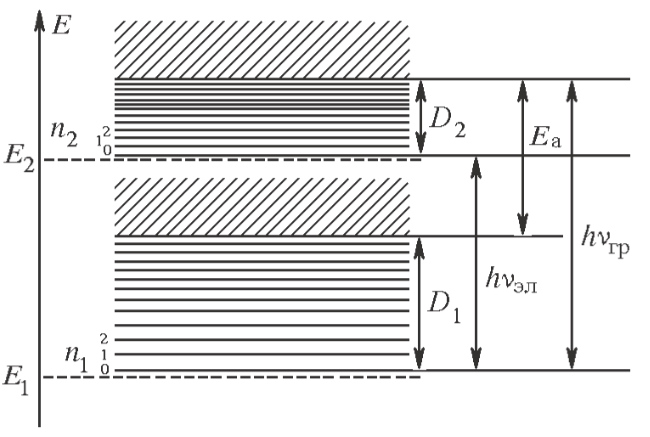
\includegraphics[width = 0.7\textwidth]{Two-atom molecule energy levels.png}
    \caption{Электронные и электронно-колебательные энергетические уровни двухатомной молекулы}
\end{figure}
На рис. \hyperref[fig: Two-atom molecule energy levels]{2} штриховыми линиями показаны чисто электронные уровни $E_1$ и
$E_2$ , а сплошными -- колебательные подуровни этих состояний. С ростом квантовых чисел $n_1$ и $n_2$ из-за ангармонизма колебательные подуровни сближаются и переходят в непрерывный спектр, области которого на рисунке заштрихованы. С
ростом $n$ растет амплитуда колебаний, при достижении некоторой максимальной амплитуды происходит разрыв связи между атомами, т. е. диссоциация молекулы.

Наименьшая энергия, которую нужно сообщить молекуле в нижайшем колебательном состоянии ($n = 0$), чтобы она диссоциировала, называется энергией диссоциации. Энергии диссоциации молекулы из состояний $n_1 = 0$ и $n_2 = 0$ обозначим через $D_1$ и $D_2$ (рис. \hyperref[fig: Two-atom molecule energy levels]{2}). На этом рисунке $E_a$ -- энергия возбуждения атома, возникающая при переходе молекулы из состояния $1$ в область непрерывного спектра, соответствующего состоянию $2$. Энергия чисто электронного перехода $E_2 - E_1 = h\nu_\text{эл}$ . Границу схождения спектра обозначим через $h\nu_\text{гр}$.

Рассмотрим теперь структуру электронно-колебательного спектра поглощения молекул йода, который исследуется в данной работе. Все возможные линии поглощения для переходов между колебательными уровнями, налагающимися на два соседних электронных состояния, можно разбить на серии, соответствующие одному и тому же начальному состоянию, как это показано на рис. \hyperref[fig: Iodine spectrum]{3}. Такие серии называются сериями Деландра. На рис. \hyperref[fig: Iodine spectrum]{3} переходы, показанные стрелками, сгруппированы соответственно в нулевую, первую и вторую серии
\begin{figure}[H]\label{fig: Iodine spectrum}
    \centering
    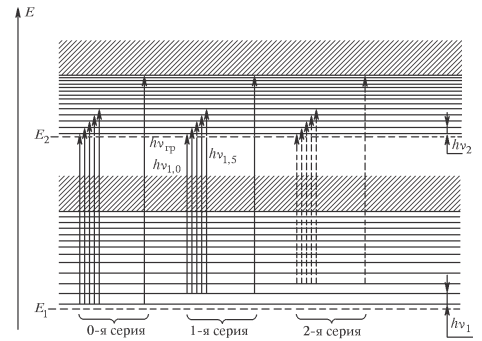
\includegraphics[width = 0.8\textwidth]{Iodine spectrum.png}
    \caption{Структура электронно-колебательного спектра поглощения молекулы йода в видимой области}
\end{figure}
Деландра. Для того чтобы в спектре поглощения наблюдалась данная серия, необходимо, чтобы в начальном состоянии ($n = 0, 1, 2, . . .$) было достаточно большое число молекул. В состоянии термодинамического равновесия число молекул $N$ в данном колебательном состоянии согласно распределению Больцмана пропорционально $\exp{-E/kT}$ , где $E$ -- энергия данного электронно-колебательного состояния, $k$ -- постоянная Больцмана, $T$ -- абсолютная температура. Соотношения интенсивностей
нулевой, первой и второй серий Деландра должны быть пропорциональны числу молекул $N_0$ , $N_1$ , $N_2$ в состояниях с $n = 0, 1, 2$.

При $T \approx 300$ K имеем
\begin{equation}\label{eq: Moleules in different states ratio}
    N_0 : N_1 : N_2 \approx 1 : \frac{1}{3} : \frac{1}{10}.
\end{equation}
Таким образом, наиболее интенсивной оказывается 0-я серия; 1-я серия примерно в 3 раза слабее, а остальные серии практически не наблюдаются.

\subsection{Общий вид спектра поглощения}
Из рассмотренного ясно, что спектр поглощения паров йода в видимой области при температуре $T \approx 300$ K практически состоит из двух серий Деландра (1-й и 0-й), накладывающихся друг на друга.
\begin{figure}[H]\label{fig: Iodine spectrum lines 0 1}
    \centering
    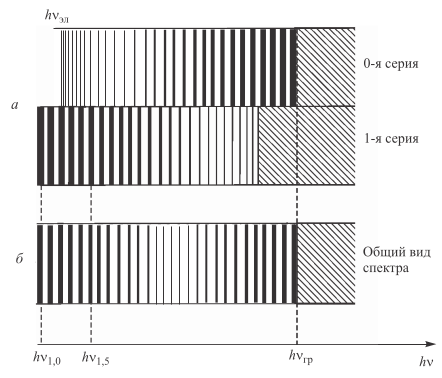
\includegraphics[width = 0.8\textwidth]{Iodine spectrum lines 0 1.png}
    \caption{Спектр поглощения паров йода}
\end{figure}

Интенсивность линии 0-й серии растет с ростом $n$, а интенсивность линий 1-й серии с ростом $n$ падает. В результате
такого распределения интенсивности поглощения в сериях с «красной» стороны (в начале спектра) видны только линии 1-й серии, а к границе сходимости линий достаточно интенсивны только линии 0-й серии. В средней части спектра наложение обеих серий приводит к «размазыванию» спектра. Расстояние между колебательными полосами уменьшается по мере приближения к «фиолетовому» концу спектра, переходя в область сплошного поглощения.

\section{Экспериментальная установка}
\begin{wrapfigure}[17]{r}{0.5\textwidth}\label{fig: Exp setup}
    \begin{center}
    \vspace{-20pt}
        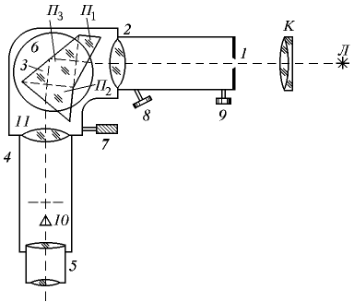
\includegraphics[width = 0.8\textwidth]{Exp setup.png}
    \end{center}
    \caption{Схематическая изображение тиратрона (слева) и его конструкция (справа): $1$, $2$, $3$ -- сетки; $4$ -- внешний металлический цилиндр; $5$ -- катод; $6$ -- анод; $7$ -- накаливаемая спираль}
\end{wrapfigure}
Для измерения длин волн спектральных линий в работе используется стеклянно-призменный монохроматор-спектрометр УМ-2, предназначенный для спектральных исследований в диапазоне от $0,38$ до $1,00$ мкм.

\subsection{Водородная лампа}
В опытах по измерению длин волн бальмеровской серии источником света служит водородная трубка $H$-образной формы, питаемая от источника высокого напряжения. 

Для увеличения яркости интересующих нас линий атомарного водорода в состав газа, которым заполняют трубку при её  изготовлении, добавляют пары воды. Молекулы воды разлагаются, образуя атомарный водород. Трубка заполняется газом до давления $5-10$ Торр.

В спектре водородной лампы также наблюдается спектр молекулярного водорода. Однако интенсивность молекулярных линий значительно слабее. 

\subsection{Изучение молекулярного спектра йода}
В данной работе спектр поглощения паров йода наблюдается визуально на фоне сплошного спектра лампы накаливания, питаемой от блока питания.

Кювета с кристаллами йода подогревается нихромовой спиралью. В результате подогрева кристаллы йода частично возгоняются, образуя пары с лёгкой фиолетовой окраской. Спектрометр позволяет визуально наблюдать линии поглощения молекул йода на фоне сплошного спектра излучения лампы накаливания видимой области.      

\section{Обработка данных}
Погрешность измерений отсчёта на барабане составляет $\Delta\theta = 1\degree$.
\subsection{Градуировка спектрометра}
Первым делом по известным спектрам неона и ртути проградуируем спектрометр. Будем измерять отсчётное значение на барабане для нескольких линий из спектра.

\begin{enumerate}
    \item 
    Измерим положение спектральных линий неона. Результаты измерений приведены в таблице ниже.
    \begin{table}[H]\label{tab: Ne data}
        \caption{Данные измерения спектра неона}
        \begin{tabular}{|
            >{\columncolor[HTML]{FFFFFF}}c |
            >{\columncolor[HTML]{FFFFFF}}c |
            >{\columncolor[HTML]{FFFFFF}}c |
            >{\columncolor[HTML]{FFFFFF}}c |
            >{\columncolor[HTML]{FFFFFF}}c |
            >{\columncolor[HTML]{FFFFFF}}c |}
            \hline
            {\color[HTML]{000000} №} &
              {\color[HTML]{000000} \begin{tabular}[c]{@{}c@{}}Отсчёт на \\ барабане, $\degree$\end{tabular}} &
              {\color[HTML]{000000} $\lambda$, \AA} &
              {\color[HTML]{000000} №} &
              {\color[HTML]{000000} \begin{tabular}[c]{@{}c@{}}Отсчёт на \\ барабане, $\degree$\end{tabular}} &
              {\color[HTML]{000000} $\lambda$, \AA} \\ \hline
            {\color[HTML]{000000} 1} &
              {\color[HTML]{000000} 2972} &
              {\color[HTML]{000000} 7245,17} &
              {\color[HTML]{000000} 9} &
              {\color[HTML]{000000} 2694} &
              {\color[HTML]{000000} 6163,59} \\ \hline
            {\color[HTML]{000000} 2} &
              {\color[HTML]{000000} 2943} &
              {\color[HTML]{000000} 7173,94} &
              {\color[HTML]{000000} 10} &
              {\color[HTML]{000000} 2664} &
              {\color[HTML]{000000} 6143,06} \\ \hline
            {\color[HTML]{000000} 3} &
              {\color[HTML]{000000} 2868} &
              {\color[HTML]{000000} 7032,41} &
              {\color[HTML]{000000} 11} &
              {\color[HTML]{000000} 2638} &
              {\color[HTML]{000000} 6074,34} \\ \hline
            {\color[HTML]{000000} 4} &
              {\color[HTML]{000000} 2839} &
              {\color[HTML]{000000} 6929,47} &
              {\color[HTML]{000000} 12} &
              {\color[HTML]{000000} 2608} &
              {\color[HTML]{000000} 5975,53} \\ \hline
            {\color[HTML]{000000} 5} &
              {\color[HTML]{000000} 2806} &
              {\color[HTML]{000000} 6598,95} &
              {\color[HTML]{000000} 13} &
              {\color[HTML]{000000} 2572} &
              {\color[HTML]{000000} 5944,83} \\ \hline
            {\color[HTML]{000000} 6} &
              {\color[HTML]{000000} 2764} &
              {\color[HTML]{000000} 6402,25} &
              {\color[HTML]{000000} 14} &
              {\color[HTML]{000000} 2526} &
              {\color[HTML]{000000} 5852,49} \\ \hline
            {\color[HTML]{000000} 7} &
              {\color[HTML]{000000} 2739} &
              {\color[HTML]{000000} 6382,99} &
              {\color[HTML]{000000} 15} &
              {\color[HTML]{000000} 2477} &
              {\color[HTML]{000000} 5656,66} \\ \hline
            {\color[HTML]{000000} 8} &
              {\color[HTML]{000000} 2714} &
              {\color[HTML]{000000} 6266,49} &
              {\color[HTML]{000000} } &
              {\color[HTML]{000000} } &
              {\color[HTML]{000000} } \\ \hline
        \end{tabular}
    \end{table}

    \item
    Теперь проведём ту же самую процедуру с ртутью. Данные представлены в таблице ниже.
    \begin{table}[H]\label{tab: Hg data}
        \caption{Данные измерения спектра ртути}
        \begin{tabular}{|
            >{\columncolor[HTML]{FFFFFF}}c |
            >{\columncolor[HTML]{FFFFFF}}c |
            >{\columncolor[HTML]{FFFFFF}}c |
            >{\columncolor[HTML]{FFFFFF}}c |
            >{\columncolor[HTML]{FFFFFF}}c |
            >{\columncolor[HTML]{FFFFFF}}c |}
            \hline
            {\color[HTML]{000000} №} &
              {\color[HTML]{000000} \begin{tabular}[c]{@{}c@{}}Отсчёт на \\ барабане, $\degree$\end{tabular}} &
              \cellcolor[HTML]{FFFFFF}{\color[HTML]{000000} $\lambda$, \AA} &
              {\color[HTML]{000000} №} &
              {\color[HTML]{000000} \begin{tabular}[c]{@{}c@{}}Отсчёт на \\ барабане, $\degree$\end{tabular}} &
              {\color[HTML]{000000} $\lambda$, \AA} \\ \hline
            {\color[HTML]{000000} 1} &
              {\color[HTML]{000000} 2502} &
              {\color[HTML]{000000} 5709,66} &
              {\color[HTML]{000000} 7} &
              {\color[HTML]{000000} 1889} &
              {\color[HTML]{000000} 4339,22} \\ \hline
            {\color[HTML]{000000} 2} &
              {\color[HTML]{000000} 2488} &
              {\color[HTML]{000000} 5789,66} &
              {\color[HTML]{000000} 8} &
              {\color[HTML]{000000} 1205} &
              {\color[HTML]{000000} 4077,83} \\ \hline
            {\color[HTML]{000000} 3} &
              {\color[HTML]{000000} 2437} &
              {\color[HTML]{000000} 5769,60} &
              {\color[HTML]{000000} 9} &
              {\color[HTML]{000000} 1186} &
              {\color[HTML]{000000} 4046,56} \\ \hline
            {\color[HTML]{000000} 4} &
              {\color[HTML]{000000} 2308} &
              {\color[HTML]{000000} 5460,73} &
              {\color[HTML]{000000} 10} &
              {\color[HTML]{000000} 709} &
              {\color[HTML]{000000} 3906,37} \\ \hline
            {\color[HTML]{000000} 5} &
              \cellcolor[HTML]{FFFFFF}{\color[HTML]{000000} 1978} &
              {\color[HTML]{000000} 4358,33} &
              {\color[HTML]{000000} 11} &
              {\color[HTML]{000000} 640} &
              {\color[HTML]{000000} 3801,66} \\ \hline
            {\color[HTML]{000000} 6} &
              \cellcolor[HTML]{FFFFFF}{\color[HTML]{000000} 1920} &
              {\color[HTML]{000000} 4347,49} &
              {\color[HTML]{000000} } &
              \cellcolor[HTML]{FFFFFF}{\color[HTML]{000000} } &
              \cellcolor[HTML]{FFFFFF}{\color[HTML]{000000} } \\ \hline
        \end{tabular}
    \end{table}

\end{enumerate}

По результатам измерения положения спектральных линий найдём зависимость $\lambda(\theta)$ -- длины волны излучения от значения на барабане спектрометра. Для этого используем формулу
\begin{equation}\label{eq: Lambda via theta}
    \fbox{\lambda = \lambda_0 + \frac{a}{\theta_0 - \theta}}
\end{equation}
где $\lambda_0$, $\theta_0$, $a$ -- константы, подлежащие определению из наилучшей аппроксимации.
\begin{table}[H]\label{tab: Consts results}
        \centering
        \begin{tabular}{|
        >{\columncolor[HTML]{FFFFFF}}c |
        >{\columncolor[HTML]{FFFFFF}}c |
        >{\columncolor[HTML]{FFFFFF}}c |
        >{\columncolor[HTML]{FFFFFF}}c |}
        \hline
        {\color[HTML]{000000} } &
          {\color[HTML]{000000} $\lambda_0$, \AA} &
          {\color[HTML]{000000} $\theta_0$, \AA} &
          {\color[HTML]{000000} $a$, отн. ед.} \\ \hline
        {\color[HTML]{000000} Значение} &
          {\color[HTML]{000000} 2143,5} &
          {\color[HTML]{000000} 3951,9} &
          {\color[HTML]{000000} 5151013} \\ \hline
        {\color[HTML]{000000} Погрешность} &
          {\color[HTML]{000000} 302,0} &
          {\color[HTML]{000000} 146,9} &
          {\color[HTML]{000000} 983811} \\ \hline
    \end{tabular}
    \caption{Результаты вычисления коэффициентов }
\end{table}
Погрешность вычисления $\lambda_0$ и $\theta_0$ не превышает $14$\%, погрешность определения $a$ составляет $19$\%.  

\subsection{Спектр водорода}
Изучим спектр водорода. Для этого
\begin{enumerate}
    \item 
    Для каждой из линий $H_\alpha$, $H_\beta$, $H_\gamma$, $H_\delta$ с помощью калибровочного графика определим длину волны:
    \begin{table}[H]\label{tab: H results}
        \centering
        \begin{tabular}{|
            >{\columncolor[HTML]{FFFFFF}}c |
            >{\columncolor[HTML]{FFFFFF}}c |
            >{\columncolor[HTML]{FFFFFF}}c |
            >{\columncolor[HTML]{FFFFFF}}c |
            >{\columncolor[HTML]{FFFFFF}}c |}
            \hline
            {\color[HTML]{000000} } &
              {\color[HTML]{000000} $H_\alpha$} &
              {\color[HTML]{000000} $H_\beta$} &
              {\color[HTML]{000000} $H_\gamma$} &
              {\color[HTML]{000000} $H_\delta$} \\ \hline
            {\color[HTML]{000000} $\theta$, $\degree$} &
              {\color[HTML]{000000} 2825} &
              {\color[HTML]{000000} 1830} &
              {\color[HTML]{000000} 1171} &
              {\color[HTML]{000000} 754} \\ \hline
            {\color[HTML]{000000} $\lambda$, \AA} &
              {\color[HTML]{000000} 6714,65} &
              {\color[HTML]{000000} 4571,13} &
              {\color[HTML]{000000} 3995,84} &
              {\color[HTML]{000000} 3754,30} \\ \hline
        \end{tabular}
        \caption{Результаты для спектральных линий водорода}
    \end{table}

    \item 
    По данным из таблицы определим постоянную Ридберга $R_y$ для каждой из линий, а также среднюю.
    \begin{table}[H]\label{tab: R_y value}
        \centering
        \begin{tabular}{|
            >{\columncolor[HTML]{FFFFFF}}c |
            >{\columncolor[HTML]{FFFFFF}}c |
            >{\columncolor[HTML]{FFFFFF}}c |
            >{\columncolor[HTML]{FFFFFF}}c |
            >{\columncolor[HTML]{FFFFFF}}c |}
            \hline
            {\color[HTML]{000000} } &
              {\color[HTML]{000000} $H_\alpha$} &
              {\color[HTML]{000000} $H_\beta$} &
              {\color[HTML]{000000} $H_\gamma$} &
              {\color[HTML]{000000} $H_\delta$} \\ \hline
            {\color[HTML]{000000} $R_y$, эВ} &
              {\color[HTML]{000000} $13,31 \pm 3,31$} &
              {\color[HTML]{000000} $14,48 \pm 3,62$} &
              \cellcolor[HTML]{FFFFFF}{\color[HTML]{000000} $14,79\pm 3,70$} &
              \cellcolor[HTML]{FFFFFF}{\color[HTML]{000000} $14,88 \pm 3,72$} \\ \hline
        \end{tabular}
        \caption{Значения постоянной Ридберга для каждой из линий}
    \end{table}
    $$
        \fbox{R_y = 14,37 \pm 1,8 \text{ эВ}} 
    $$
    Полученный результат совпадает с табличным значением $R = 13,6 \text{ эВ}$ в пределах  
    погрешности.
\end{enumerate}

\subsection{Спектр йода}
\begin{enumerate}
    \item 
    Измерим значения длин волн линий поглощения йода.
    \begin{table}[H]\label{tab: I data}
        \centering
        \begin{tabular}{|
            >{\columncolor[HTML]{FFFFFF}}c |
            >{\columncolor[HTML]{FFFFFF}}c |
            >{\columncolor[HTML]{FFFFFF}}c |
            >{\columncolor[HTML]{FFFFFF}}c |}
            \hline
            {\color[HTML]{000000} } &
              {\color[HTML]{000000} $n_{1,0}$} &
              {\color[HTML]{000000} $n_{1,5}$} &
              {\color[HTML]{000000} $n_\text{гран.}$} \\ \hline
            {\color[HTML]{000000} $\lambda$, \AA} &
              \cellcolor[HTML]{FFFFFF}{\color[HTML]{000000} 5867} &
              {\color[HTML]{000000} 5697} &
              {\color[HTML]{000000} 5049} \\ \hline
            {\color[HTML]{000000} $h\nu$, эВ} &
              {\color[HTML]{000000} 2,12} &
              {\color[HTML]{000000} 2,18} &
              {\color[HTML]{000000} 2,46} \\ \hline
        \end{tabular}
        \caption{Результаты измерения линий  спектра йода}
    \end{table}

    \item 
    Теперь рассчитаем энергию колебательного кванта возбуждённого состояния молекулы йода:
    $$
        h\nu_2 = (h\nu_{1,5} - h\nu_{1,0}) / 5 = 0,012 \text{ эВ}.
    $$

    \item 
    Затем посчитаем энергию диссоциации молекулы в основном состоянии $D_1$, энергию диссоциации молекулы в возбужденном состоянии $D_2$ и энергию электронного перехода $h\nu_\text{эл.}$, полагая  $h\nu_1 = 0,027$ эВ -- энергия колебательного кванта основного состояния, $E_a = 0,94$ эВ -- энергия возбуждения атома. Получаем
    $$
        D_1 \approx 1,52 \text{ эВ},\; D_2 \approx 0,31 \text{ эВ},\; \Delta E \approx 2,14 \text{ эВ} 
    $$
    
\end{enumerate}

\newpage
\section{Вывод}
В данной работе исследовалоись спетральные линии излучения атомов водорода и молекул йода. В результате удалось:
\begin{itemize}
    \item
    по известным длинам волн для излучения неона и ртути получить зависимость длины волны от отсчётного значения на барабане установки
    \item
    измерить спектральные линии $H_\alpha$, $H_\beta$, $H_\gamma$, $H_\delta$ водорода. По полученным значениям рассчитать постоянную Ридберга, которая оказалась равна $R_y = 14,37 \pm 1,8$ эВ, что в пределах погрешности совпало с истинным значением $R = 13,6$ эВ
    \item
    изучить спектр излучения молекул йода. По экспериментальным данным вычислить энергии диссоциации молекулы йода в основном и возбуждённом состояниях $D_1 \approx 1,52 \text{ эВ},\; D_2 \approx 0,31 \text{ эВ}$ соответственно, а также вычислить энергию возбуждения атома $\Delta E \approx 2,14 \text{ эВ}$. 
    
\end{itemize}

\newpage
%%%%%%%%%%%%%%%%%%%%%%%%% Графики
\begin{figure}[H]\label{fig: lambd via degree}
    \centering
    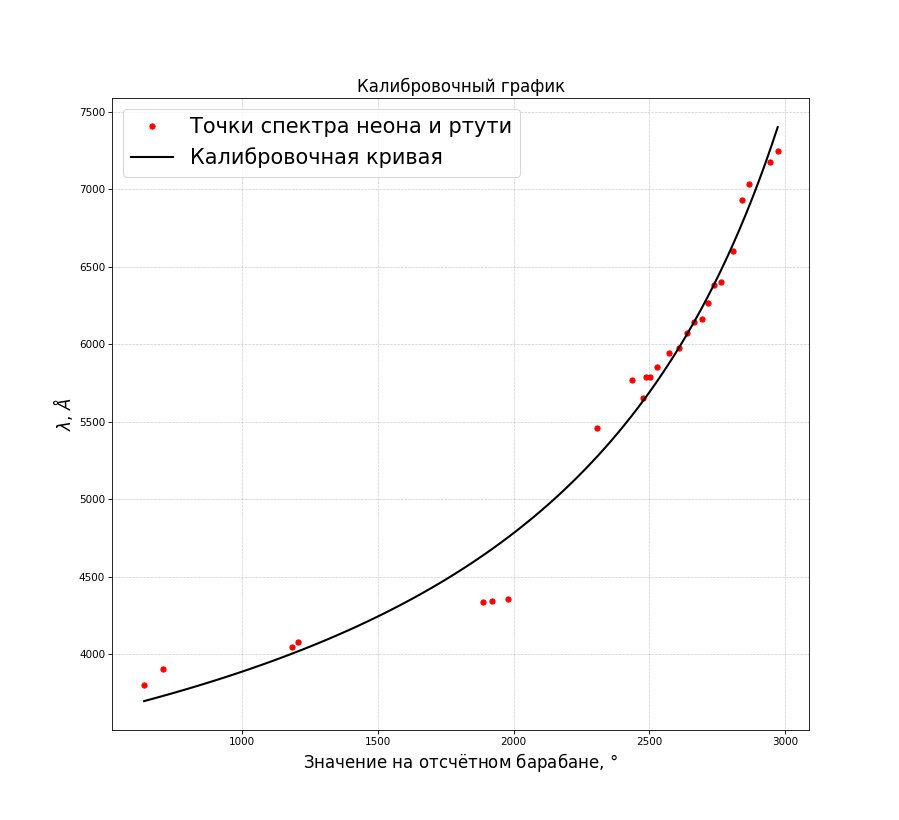
\includegraphics[width = \textwidth]{lambd(deg).png}
\end{figure}

%%%%%%%%%%%%%%%%%%%%%%%%%
\end{document}
